%% ---------------------------------------------------------------------------
%% This file is part of the "Boost Python" talk.
%%
%% Copyright 2015 by Eugen Wintersberger <eugen.wintersberger@gmail.com>
%%
%% This work is licensed under the Creative Commons
%% Attribution-NonCommercial-ShareAlike 4.0 International License. To view 
%% a copy of this license, visit 
%% http://creativecommons.org/licenses/by-nc-sa/4.0/.
%% ---------------------------------------------------------------------------
\documentclass{beamer}
\usepackage{tikz}
\usepackage{pgfpages}
\usepackage{todonotes}
\usepackage{array}
\usepackage{multirow}
\usepackage{hyperref}
\usepackage{copyrightbox}
\usepackage{minted}
\usepgflibrary{shapes.multipart}
\usepgflibrary{shapes.symbols}
\usetikzlibrary{positioning}
\usetikzlibrary{calc}
\usetikzlibrary{fit}
\usetikzlibrary{datavisualization}


\setbeamercolor{frametitle}{fg=black,bg=white}
\setbeamerfont{frametitle}{series=\bfseries}
\setbeamercolor{part page}{fg=black,bg=white}
\setbeamerfont{part page}{series=\bfseries}
\setbeamercolor{part title}{fg=black}
\setbeamercolor{part subtitle}{fg=black}
\setbeamercolor{author}{fg=white}
\setbeamercolor{date}{fg=white}



\setbeamercolor{title}{fg=black}
\setbeamerfont{title}{series=\bfseries,size=\Huge}
\setbeamercolor{subtitle}{fg=black}

\setbeamercolor{item}{fg=black}


%\setbeameroption{show notes on second screen}

\title{{\Huge Boost Python}}
\subtitle{From C++ to Python and back}
\author{Eugen Wintersberger\\ \small{eugen.wintersberger@gmail.com}}
\date{January 19, 2016}

\begin{document}

%%%===========================================================================
\frame{\titlepage}
\part{Motivation}
\section{Motivation}

\frame{\partpage }
\begin{frame}[fragile]{Why mixing C++ and Python? - Two use cases}
    \note{
        \begin{itemize}
            \item \texttt{Ipython}-session loading a C++ wrapper
            \item Paraview uses Python as its internal scripting language
        \end{itemize}
        Only C++ from python will be covered in this talk.
    }
    \begin{center}
        \textbf{Calling C++ from python}
    \end{center}
    \begin{columns}[c]
        \begin{column}{0.49\linewidth}
            \begin{itemize}
                \item write performance critical code in C++
                \item reuse existing C++ libraries 
            \end{itemize}
        \end{column}
        \hfill
        \begin{column}{0.4\linewidth}
            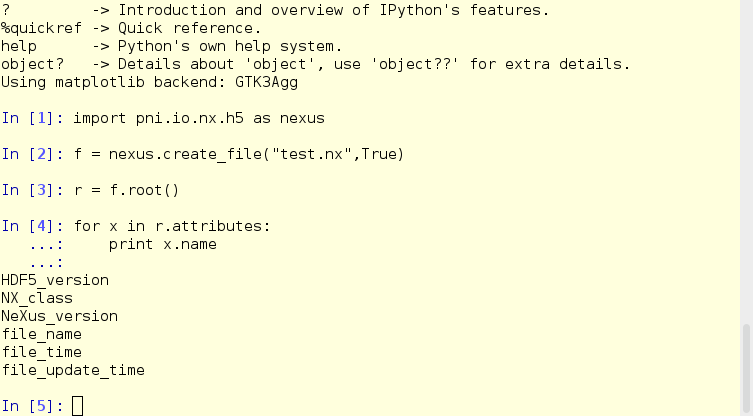
\includegraphics[width=\linewidth]{pics/ipython_screenshot.png}
        \end{column}
    \end{columns}
    
    \vspace{0.05\textheight}
    \begin{center}
        \textbf{Calling Python from C++}
    \end{center}
    \begin{columns}[c]
        \begin{column}{0.49\linewidth}
            Use Python as an embedded scripting language for a 
            C++ application
        \end{column}
        \hfill
        \begin{column}{0.4\linewidth}
            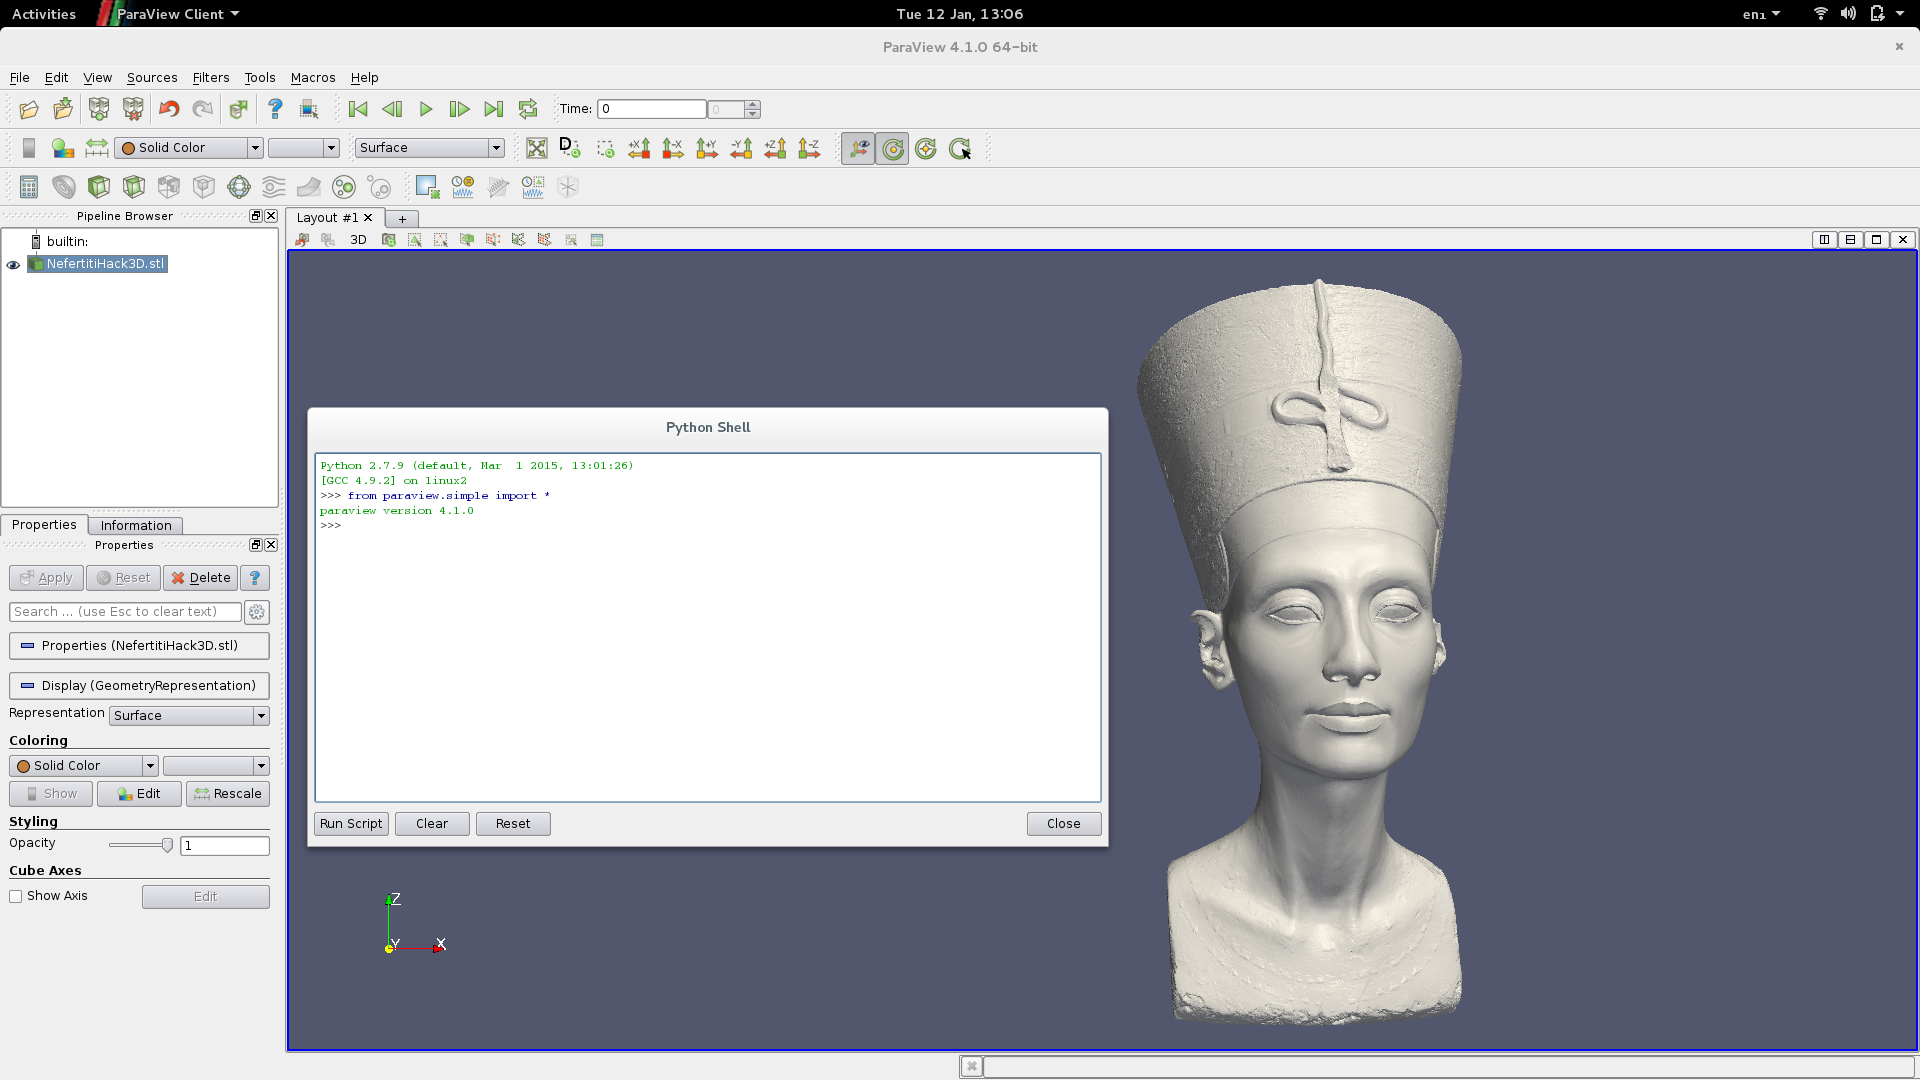
\includegraphics[width=\linewidth]{pics/paraview.png}
        \end{column}
    \end{columns}
    

\end{frame}

%%%===========================================================================
\begin{frame}[fragile]{Available technologies}
    \note{
        Our focus is on \texttt{boost::python}!
    }
    
    \begin{itemize}
        \setlength{\itemsep}{0.075\textheight}
        \item native Python C-API (do not use this until you have to)
        \item \texttt{boost::python} (part of the BOOST distribution)
        \item \texttt{cython} -- good for numerical applications
        \item \texttt{sheboken} -- used for instance with \texttt{pyside}
    \end{itemize}
\end{frame}



%%%===========================================================================
\part{\texttt{boost::python}}
\section{boost::python}
\frame{\partpage}


%%%---------------------------------------------------------------------------
\begin{frame}[fragile]{Building \texttt{boost::python} package}
    Directory layout of a project
    \begin{center}
        \begin{tabular}{ll}
            \texttt{setup.py} & script to finally run the build \\
            \texttt{src/}     & directory with C++ source files \\
            \texttt{talk/}    & directory with Python code of the package \\
            \texttt{talk/test/}    & Python unit tests \\
        \end{tabular}
    \end{center}
    \vspace{0.05\textheight}
    \texttt{boost::python} modules are built like any other non-native 
    Python package with C extensions by means of \texttt{setup.py}
    \vspace{0.05\textheight}
    \begin{minted}{bash}
$ python setup.py install --user 
    \end{minted}
    or 
    \begin{minted}{bash}
$ python3 setup.py install --user
    \end{minted}
\end{frame}

%%%---------------------------------------------------------------------------
\begin{frame}[fragile]{The \texttt{setup.py} file}
    \begin{minted}[fontsize=\tiny]{python}
#setup script for python-talk
from __future__ import print_function
import sys
import os
from setuptools import setup, find_packages, Extension

boost_python_lib = 'boost_python-py{version[0]}{version[1]}'.format(version=sys.version_info)

extra_compile_args = ['-std=c++11','-Wall','-Wextra',
                      '-fdiagnostics-show-option',
                      '-Wno-strict-prototypes']

functions_ext = Extension("talk.functions",
                          ["src/functions.cpp"],
                          libraries = ["talk",boost_python_lib],
                          language="c++",
                          extra_compile_args = extra_compile_args)

setup(name="talk",
      author="Eugen Wintersberger",
      author_email="eugen.wintersberger@gmail.com",
      description="Python wrapper for the talk library",
      maintainer = "Eugen Wintersberger",
      maintainer_email = "eugen.wintersberger@gmail.com",
      license = "GPLv2",
      version = "1.0.0",
      ext_modules=[functions_ext,test_exceptions_ext,sensor_ext,motors_ext],
      packages = find_packages(),
      test_suite="talk.test",
      test_loader = "unittest:TestLoader",
    )
    \end{minted}
\end{frame}

%%%---------------------------------------------------------------------------
\begin{frame}[fragile]{C++ functions to Python}
    \begin{center}
        \begin{tikzpicture}
            \node (filename) {\texttt{talk/functions.hpp}};
            \node[draw,black,rectangle,below = 0.2cm of filename]
            (header file)
            {
                \begin{minipage}{0.4\linewidth}
    \inputminted[fontsize=\tiny,firstline=23,firstnumber=23]{cpp}
    {../src/libtalk/include/talk/functions.hpp}
    \end{minipage}
            };

            \onslide<2->
            \node[right = 1cm of filename]  (wrap simple) {wrapping unique function};
            \node[draw,rectangle,below = 0.2cm of wrap simple]
            {
                \begin{minipage}{0.35\linewidth}
                    \begin{minted}[fontsize=\tiny]{cpp}
#include <boost/python.hpp>
#include <talk/functions.hpp>

using namespace boost::python;

BOOST_PYTHON_MODULE(functions)
{
    def("div",talk::div);
}
                    \end{minted}
                \end{minipage}
            };
            
            \onslide<3->
            \node[below = 1cm of header file] (wrap overload) {wrapping overloaded functions};
            \node[rectangle,draw,below = 0.2cm of wrap overload]
            {
                \begin{minipage}{0.7\linewidth}
                    \begin{minted}[fontsize=\tiny]{cpp}
#include <boost/python.hpp>
#include <talk/functions.hpp>

using namespace boost::python;

BOOST_PYTHON_FUNCTION_OVERLOADS(add_overloads,talk::add,2,2);

BOOST_PYTHON_MODULE(functions)
{
    def("add",(double (*)(double,double))2,add_overloads());
    def("add",(int (*)(int,int))2,add_overloads());
}
                    \end{minted}
                \end{minipage}
            };
        \end{tikzpicture}
    \end{center}
\end{frame}

%%%---------------------------------------------------------------------------
\begin{frame}[fragile]{Mapping of primitive data types}
    \begin{center}
        {
            \renewcommand{\arraystretch}{1.5}
            \begin{tabular}{p{0.3\linewidth}|p{0.3\linewidth}}
            \textbf{C++ type} & \textbf{Python type} \\
            \hline
            all integer types & \texttt{int} or \texttt{long} \\
            \texttt{double} & \texttt{float} \\
            \texttt{std::string} & Python string type  \\
        \end{tabular}
    }
    \end{center}
    \vspace{0.1\textheight}
    For all other types converters are required!
\end{frame}

%%%---------------------------------------------------------------------------
\begin{frame}[fragile]{Handling exceptions}
    Two possibilities
    \vspace{0.04\textheight}
    \begin{enumerate}
        \setlength{\itemsep}{0.04\textheight}
        \item translate the C++ exception into an existing Python exception
        \item create a new Python exception in the extension modules scope
    \end{enumerate}
    \vspace{0.05\textheight}
    \begin{center}
        \textbf{The first approach is recommended and should be used whenever
        possible!}
    \end{center}

    \begin{center}
    \inputminted[fontsize=\tiny,firstline=24]{cpp}
    {../src/libtalk/include/talk/exceptions.hpp}
    \end{center}
\end{frame}

%%%---------------------------------------------------------------------------
\begin{frame}[fragile]{Handling exceptions - translation}
    A rather straight forward approach
    \vspace{0.04\textheight}
    \begin{minted}[fontsize=\tiny]{cpp}
#include <boost/python.hpp>
#include <talk/functions.hpp>
#include <talk/exceptions.hpp>

using namespace boost::python;

void division_by_zero_translator(const talk::division_by_zero &)
{
    PyErr_SetString(PyExc_ZeroDivisionError,"only Chuck Norris can do this!");
}

BOOST_PYTHON_MODULE(functions)
{
    def("div",talk::div);
    register_exception_translator<talk::division_by_zero>(division_by_zero_translator);
}
    \end{minted}
\end{frame}

%%%---------------------------------------------------------------------------
\begin{frame}[fragile]{Handling exceptions - new exception}

\begin{tikzpicture}
    \node{
        \begin{minipage}{\linewidth}
        \begin{minted}[fontsize=\tiny]{cpp}
#include <boost/python.hpp>
#include <talk/functions.hpp>
#include <talk/exceptions.hpp>

using namespace boost::python;

static object TalkError;
static char *TalkError_Doc = "Internal error in talk library";

void talk_error_translator(const talk::talk_error &)
{
    PyErr_SetString(TalkError.ptr(),"An internal error");
}

BOOST_PYTHON_MODULE(functions)
{
    TalkError = object(handle<>(PyErr_NewExceptionWithDoc("talk.functions.TalkError",TalkError_Doc,
                                                          nullptr,nullptr)));
    scope().attr("TalkError")=TalkError;

    register_exception_translator<talk::talk_error>(talk_error_translator);
   
}
        \end{minted}
        \end{minipage}
    };
%    \node[draw,thick,text width=0.2\linewidth] (static variable) at (2cm,3cm) 
%    {\small static variable for the new exception};
%    \draw[black,thick] (-2.7,1.2) -- (static variable.west);
%    
%    \node[draw,thick,text width=0.2\linewidth] (docstring) at (4cm,1.5cm) 
%    {\small doc string};
\end{tikzpicture}
\begin{enumerate}
    \item static object for the new execption and its doc string
    \item implement translation function
    \item create exception object and register it in the modules' scope
    \item register the translation function
\end{enumerate}
\end{frame}

%%%---------------------------------------------------------------------------
\begin{frame}[fragile]{C++ classes to Python}
    \begin{columns}[t]
        \begin{column}{0.4\linewidth}
            Consider a simple class 
            \inputminted[fontsize=\tiny,firstline=22]{cpp}
            {../src/libtalk/include/talk/sensor.hpp}
        \end{column}
        \hfill
        \begin{column}{0.5\linewidth}
            Wrapper code
            \begin{minted}[fontsize=\tiny]{cpp}
#include <boost/python.hpp>
#include <talk/sensor.hpp>

using namespace boost::python;

BOOST_PYTHON_MODULE(sensor)
{
    class_<talk::sensor>("Sensor")
        .def("get_value",&talk::sensor::get_value)
        .def("set_value",&talk::sensor::set_value);
}
            \end{minted}
        \end{column}
    \end{columns}
    \vspace{0.03\textheight}
    In Python we finally get something like
    \begin{minted}[fontsize=\tiny]{python}
>>> from talk import Sensor
>>> s = Sensor()
>>> s.set_value(0.23)
>>> print(s.get_value())
0.23
    \end{minted}
\end{frame}

%%%---------------------------------------------------------------------------
\begin{frame}[fragile]{Dealing with constructors}
    The C++ class has more than one constructor.
    \vspace{0.02\textheight}
    \begin{minted}[fontsize=\tiny]{cpp}
#include <boost/python.hpp>
#include <talk/sensor.hpp>

using namespace boost::python;

BOOST_PYTHON_MODULE(sensor)
{
    class_<talk::sensor>("Sensor")
        .def(init<>())
        .def(init<double>())
        .def("get_value",&talk::sensor::get_value)
        .def("set_value",&talk::sensor::set_value);
}
    \end{minted}
    \vspace{0.03\textheight}
    Get in Python
    \vspace{0.02\textheight}
    \begin{minted}[fontsize=\tiny]{python}
>>> from talk import Sensor
>>> s = Sensor()
>>> print(s.get_value())
0.0
>>> s = Sensor(2.3)
>>> print(s.get_value())
0.23
    \end{minted}
\end{frame}

%%%---------------------------------------------------------------------------
\begin{frame}[fragile]{Python properties}
    Properties are an alternative way how to access the attributes of a Python
    class 
    \vspace{0.02\textheight}
    \begin{minted}[fontsize=\tiny]{cpp}
#include <boost/python.hpp>
#include <talk/sensor.hpp>

using namespace boost::python;

BOOST_PYTHON_MODULE(sensor)
{
    class_<talk::sensor>("Sensor")
        .def(init<>())
        .def(init<double>())
        .def("get_value",&talk::sensor::get_value)
        .def("set_value",&talk::sensor::set_value)
        .add_property("value",&talk::sensor::get_value,
                          &talk::sensor::set_value); 
}
    \end{minted}
    \vspace{0.03\textheight}
    Get in Python
    \vspace{0.02\textheight}
    \begin{minted}[fontsize=\tiny]{python}
>>> from talk import Sensor
>>> s = Sensor()
>>> s.value = 12.23
>>> print(s.value)
12.23
    \end{minted}
\end{frame}

%%%---------------------------------------------------------------------------
\begin{frame}[fragile]{Dealing with inheritance}
    \only<1>{
    C++ base class
    \inputminted[fontsize=\tiny,firstline=24,lastline=45]{cpp}
{../src/libtalk/include/talk/motor.hpp}
}

\only<2>{
    C++ derived class
    \inputminted[fontsize=\tiny,firstline=26,lastline=43]{cpp}
{../src/libtalk/include/talk/step_motor.hpp}
}
\end{frame}

\begin{frame}[fragile]{Dealing with inheritance}
    Wrapper 
    \begin{minted}[fontsize=\tiny]{cpp}
#include <boost/python.hpp>
#include <talk/motor.hpp>
#include <talk/step_motor.hpp>

using namespace boost::python;

BOOST_PYTHON_MODULE(motors)
{
    class_<talk::motor>("Motor")
        .def(init<>())
        .def(init<double,double>())
        .add_property("upper_limit",&talk::motor::get_upper_limit,
                                    &talk::motor::set_upper_limit)
        .add_property("lower_limit",&talk::motor::get_lower_limit,
                                    &talk::motor::set_lower_limit)
        .add_property("position",&talk::motor::get_position);
                       

    class_<talk::step_motor,bases<talk::motor>>("StepMotor")
        .def(init<>())
        .def(init<double,double,double,double>())
        .add_property("step_size",&talk::step_motor::get_step_size,
                                  &talk::step_motor::set_step_size)
        .add_property("position",&talk::step_motor::get_position,
                                 &talk::step_motor::set_position);
}
    \end{minted}
\end{frame}






%%%===========================================================================
\part{The odds and ends}
\section{The odds and ends}
\frame{\partpage}

%%%---------------------------------------------------------------------------
\begin{frame}[fragile]{What is missing}
    \begin{enumerate}
        \item the \texttt{boost::python} C++ API
        \item handling object ownership
        \item type converters
        \item calling Python from C++
    \end{enumerate}
\end{frame}

%%%---------------------------------------------------------------------------
\begin{frame}[fragile]{Further reading}

    \begin{itemize}
        \item
            \href{http://www.boost.org/doc/libs/1_60_0/libs/python/doc/html/index.html}
            {Official Boost Python documentation}
        \item 
            \href{https://wiki.python.org/moin/boost.python}
            {Boost Python Wiki}
    \end{itemize}

\end{frame}

\end{document}
